\documentclass[12pt]{article}
\usepackage[english]{babel}
\usepackage{natbib}
\usepackage{url}
\usepackage[utf8x]{inputenc}
\usepackage{amsmath}
\usepackage{graphicx}
\graphicspath{{images/}}
\usepackage{parskip}
\usepackage{fancyhdr}
\usepackage{vmargin}
\usepackage{listings}
\usepackage[dvipsnames]{xcolor}
\setmarginsrb{3 cm}{2.5 cm}{3 cm}{2.5 cm}{1 cm}{1.5 cm}{1 cm}{1.5 cm}

\title{Team-107 Project UML Diagrams}			
\author{D.Panse, S. Sood, S. Shah,V. Dave}	
\date{April 17, 2018}							

\makeatletter
\let\thetitle\@title
\let\theauthor\@author
\let\thedate\@date
\def\thecourse{CS5500: Managing Software Development}
\def\theuniversity{Northeastern University}
\def\thecollege{College of Computer and Information Science}
\def\thegithuburl{https://github.ccs.neu.edu/cs5500/team-107}
\makeatother

\pagestyle{fancy}
\fancyhf{}
\rhead{\theauthor}
\lhead{\thetitle}
\cfoot{\thepage}

\usepackage{color}
 
\definecolor{codegreen}{rgb}{0,0.6,0}
\definecolor{codegray}{rgb}{0.5,0.5,0.5}
\definecolor{codepurple}{rgb}{0.58,0,0.82}
\definecolor{backcolour}{rgb}{0.95,0.95,0.92}
\definecolor{huskyred}{HTML}{CC0000}
\definecolor{lightgray}{gray}{0.9}

\lstset{
    showstringspaces=false,
    basicstyle=\ttfamily,
    keywordstyle=\color{blue},
    commentstyle=\color[grey]{0.6},
    stringstyle=\color[RGB]{255,150,75}
}

\newcommand{\inlinecode}[2]{\colorbox{backcolour}{\lstinline[language=#1]$#2$}}
 
\lstdefinestyle{mystyle}{
    backgroundcolor=\color{backcolour},   
    commentstyle=\color{codegreen},
    keywordstyle=\color{magenta},
    numberstyle=\tiny\color{codegray},
    stringstyle=\color{codepurple},
    basicstyle=\footnotesize,
    breakatwhitespace=false,         
    breaklines=true,                 
    captionpos=b,                    
    keepspaces=true,                 
    numbers=left,                    
    numbersep=5pt,                  
    showspaces=false,                
    showstringspaces=false,
    showtabs=false,                  
    tabsize=2
}

\lstset{style=mystyle}
 

\begin{document}

%%%%%%%%%%%%%%%%%%%%%%%%%%%%%%%%%%%%%%%%%%%%%%%%%%%%%%%%%%%%%%%%%%%%%%%%%%%%%%%%%%%%%%%%%

\begin{titlepage}
	\centering
    
\includegraphics[scale = 0.20]{seal.png}\\[0.2cm]	
    \textsc{\LARGE \color{huskyred} \theuniversity\\[0.5mm]}	
	\textsc{\small \thecollege \\[1.5 cm]}	
    
    \textsc{\Large \thecourse }\\[0.5 cm]
    
	\rule{\linewidth}{0.2 mm} \\[0.4 cm]
	{ \huge \bfseries \thetitle}\\
	\rule{\linewidth}{0.2 mm} \\[1.5 cm]
	
	\textsc{\LARGE Darshan Panse, Samanjate Sood}\\[0.5 mm]
    \textsc{\LARGE Shail Shah, Vaibhav Dave}\\[0.5 mm]
    \thegithuburl\\[1.5 cm]
    \textsc{\LARGE \thedate}\\[2.0 cm]  
    
\end{titlepage}

%%%%%%%%%%%%%%%%%%%%%%%%%%%%%%%%%%%%%%%%%%%%%%%%%%%%%%%%%%%%%%%%%%%%%%%%%%%%%%%%%%%%%%%%%

% \tableofcontents
% \pagebreak

%%%%%%%%%%%%%%%%%%%%%%%%%%%%%%%%%%%%%%%%%%%%%%%%%%%%%%%%%%%%%%%%%%%%%%%%%%%%%%%%%%%%%%%%%

Class Diagram describing the back-end system structure:\\
\begin{center}
    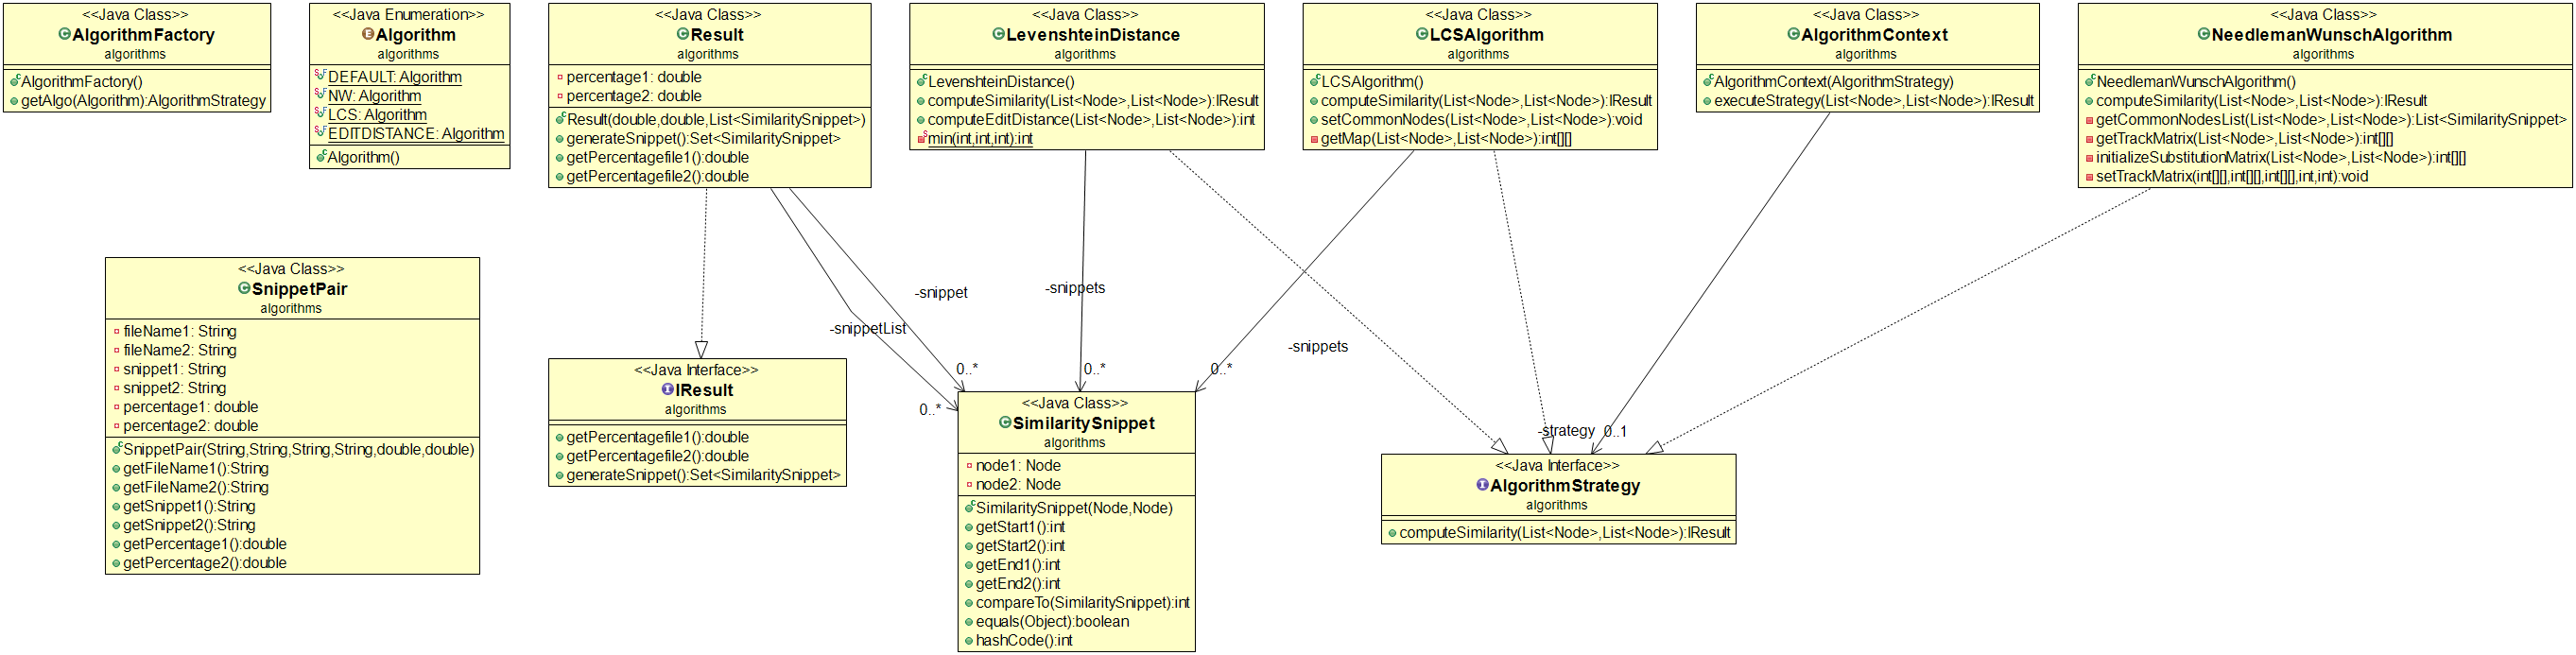
\includegraphics[scale = 0.20, angle = 90]{UML1.png}
\end{center}
\pagebreak
Class Diagram describing driver and back-end interactions:\\
\begin{center}
    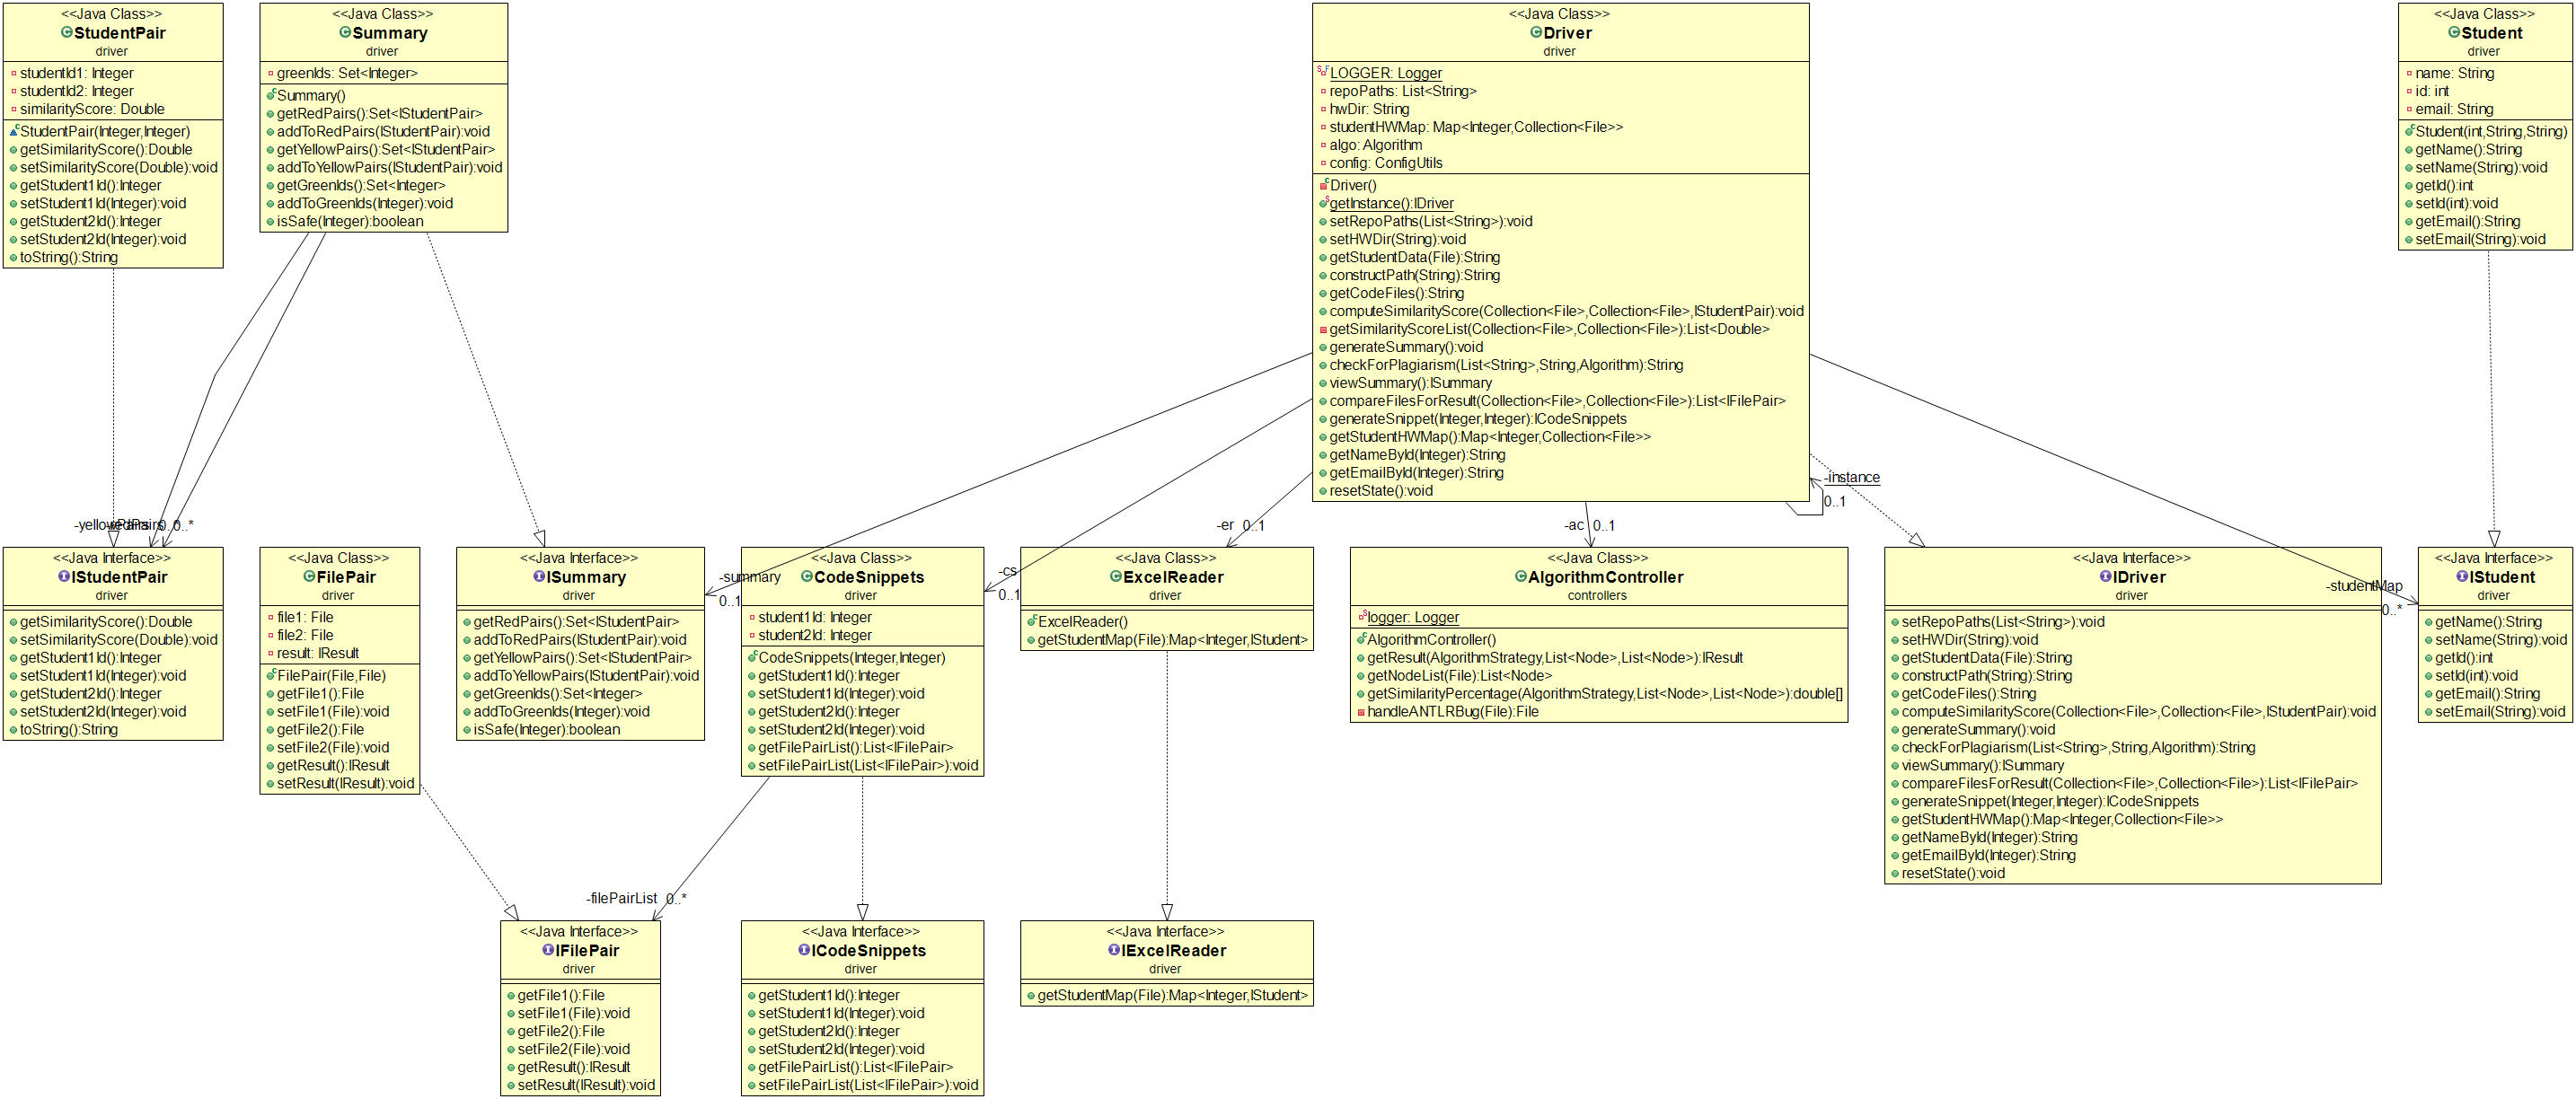
\includegraphics[scale = 0.19, angle = 90]{UML2.png}
\end{center}
\pagebreak
Class Diagram describing driver and front-end interactions:\\
\begin{center}
    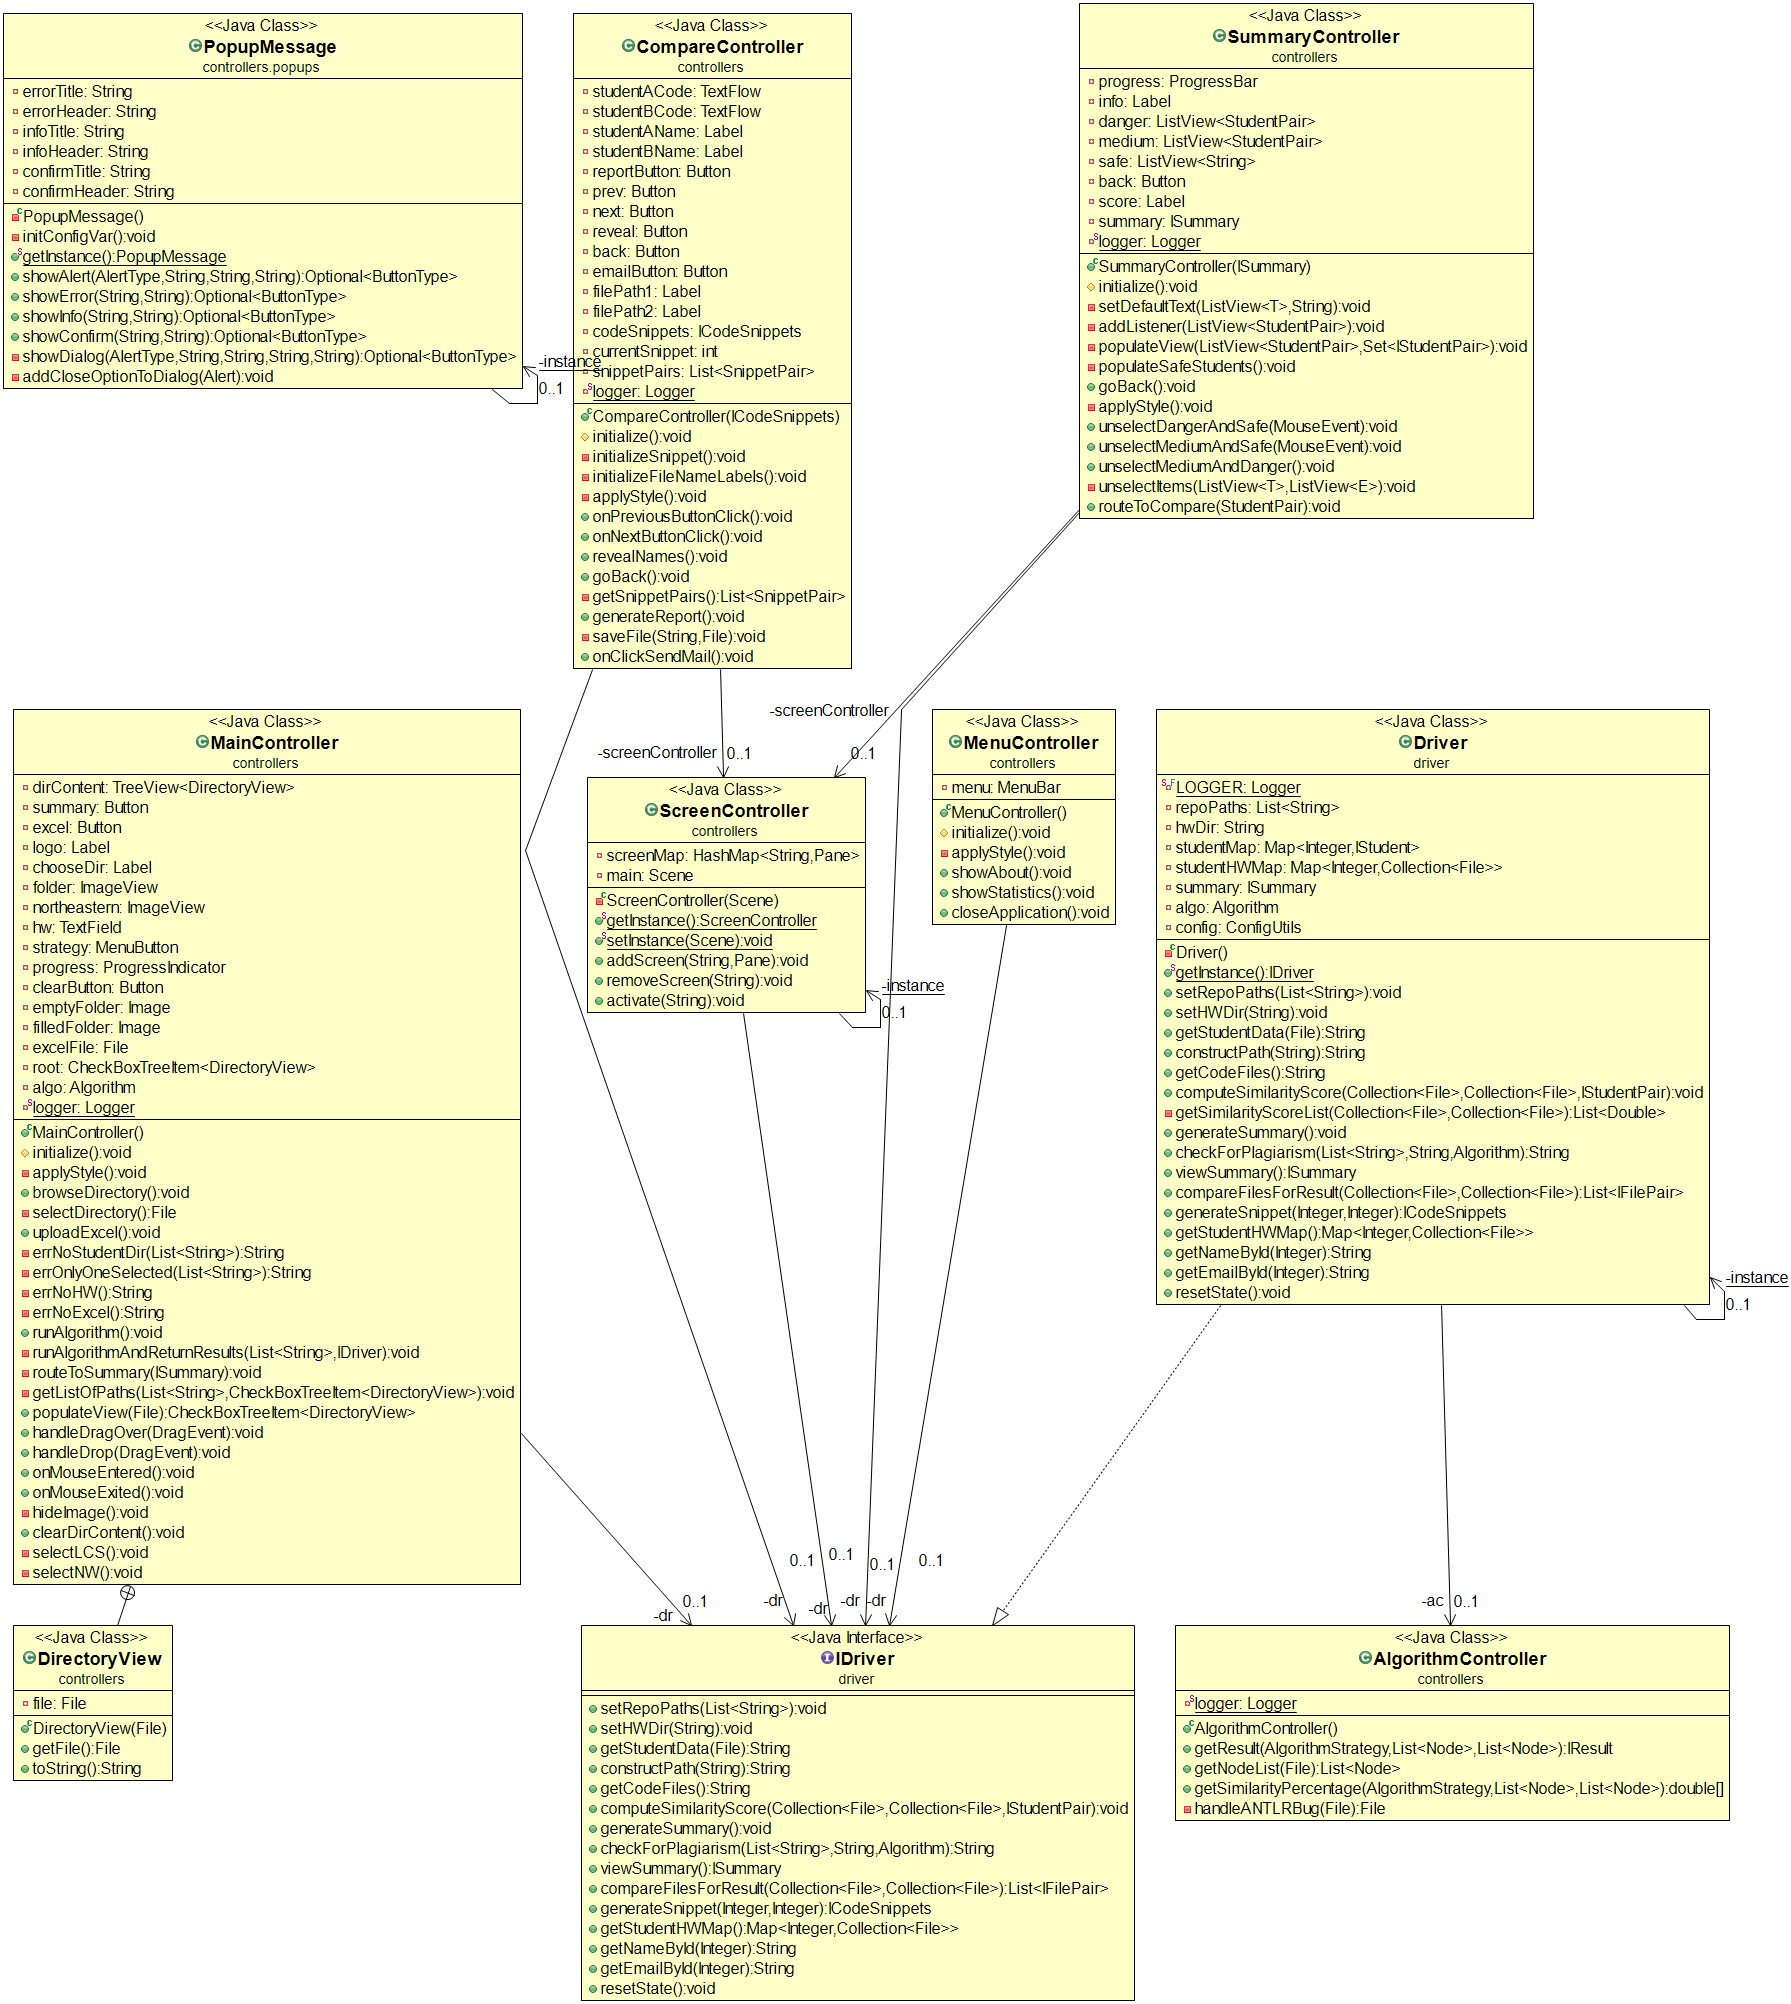
\includegraphics[scale = 0.25]{UML3.png}
\end{center}




\end{document}